\section{Auswertung}

\subsection{Teilchenidentifikation}

\begin{figure}[h]
	\centering
	\subfigure[Elektronen]{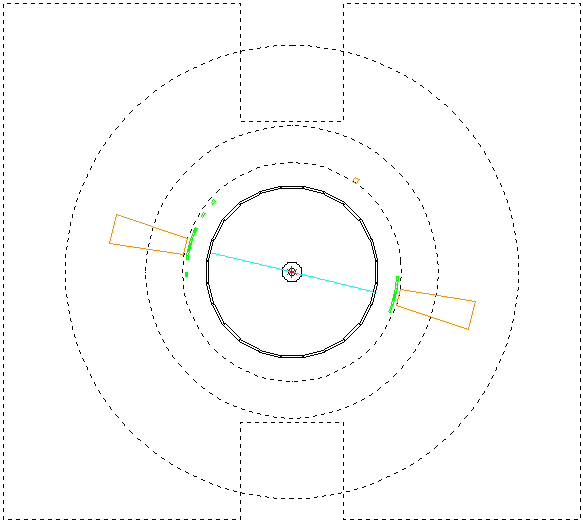
\includegraphics[width=0.49\textwidth]{../figures/grope-ee-w.png}}
	\subfigure[Myonen]{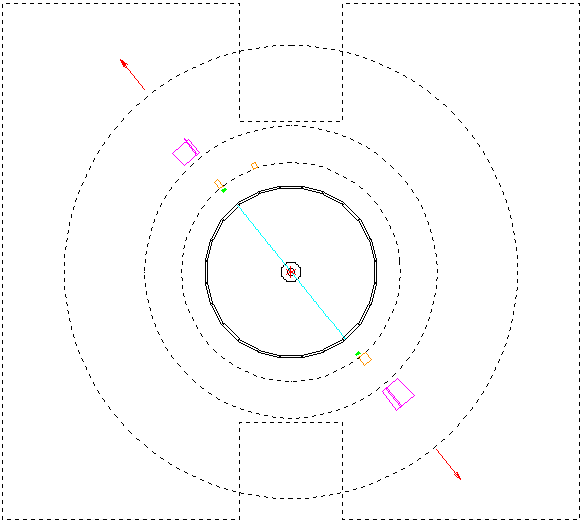
\includegraphics[width=0.49\textwidth]{../figures/grope-mm-w.png}}
	\subfigure[Tauonen]{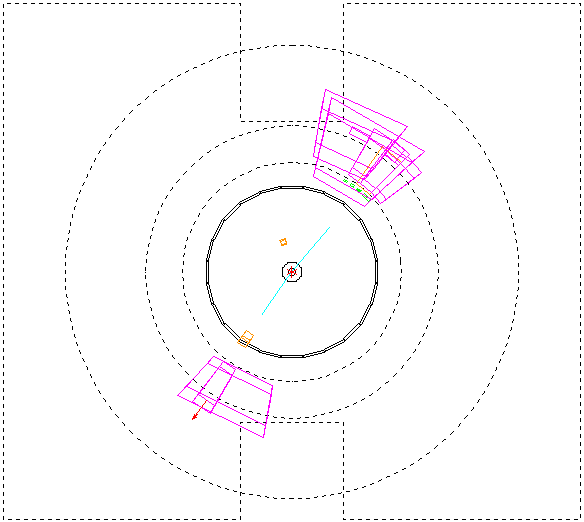
\includegraphics[width=0.49\textwidth]{../figures/grope-tt-w.png}}
	\subfigure[Quarks]{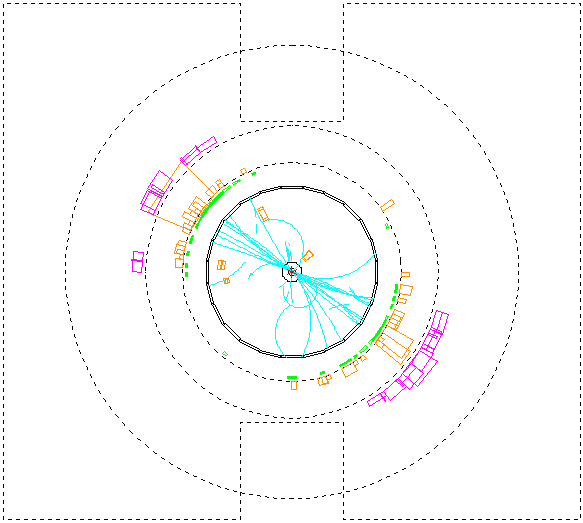
\includegraphics[width=0.49\textwidth]{../figures/grope-qq-w.png}}
	\caption[Detektor-Simulationen für die erwarteten Zerfallsprozesse des Z\textsuperscript0-Bosons]{Detektor-Simulationen für die erwarteten Zerfallsprozesse des Z\textsuperscript0-Bosons. Die Bilder wurden mit GROPE aufgenommen und mit GIMP zur besseren Sichtbarkeit bearbeitet.}
	\label{fig:grope}
\end{figure}
Um später die Separation der Zerfallskanäle durchführen zu können, werden zunächst die einzelnen Zerfallskanäle simuliert und betrachtet. In Abbildung \ref{fig:grope} ist für jeden Zerfallskanal ein Prozess beispielhaft dargestellt.

\begin{figure}[h]
	\centering
	\subfigure[$N_\mathrm{charged}$]{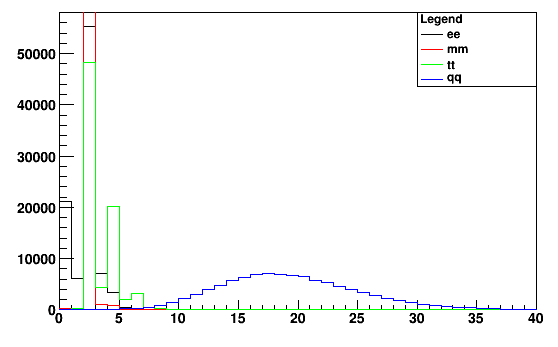
\includegraphics[width=0.49\textwidth]{../figures/Ncharged.png}}
	\subfigure[$P_\mathrm{charged}$]{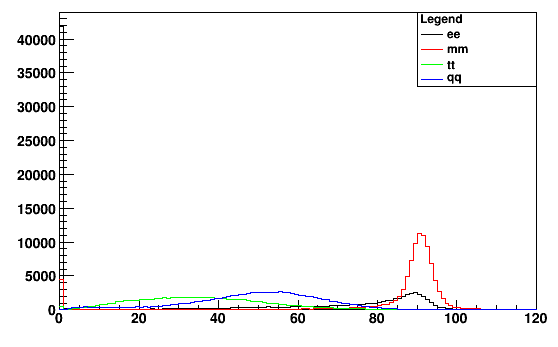
\includegraphics[width=0.49\textwidth]{../figures/Pcharged.png}}
	\subfigure[$E_\mathrm{ecal}$]{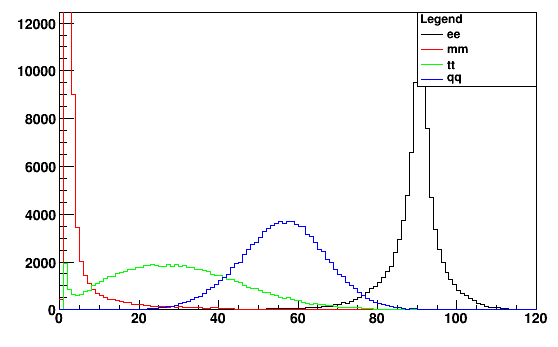
\includegraphics[width=0.49\textwidth]{../figures/E_ecal.png}}
	\subfigure[$E_\mathrm{hcal}$]{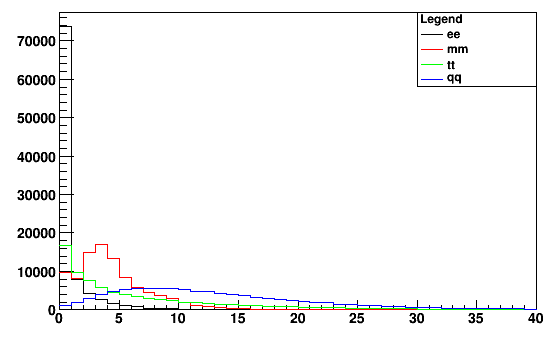
\includegraphics[width=0.49\textwidth]{../figures/E_hcal.png}}
	\subfigure[$\cos\theta$]{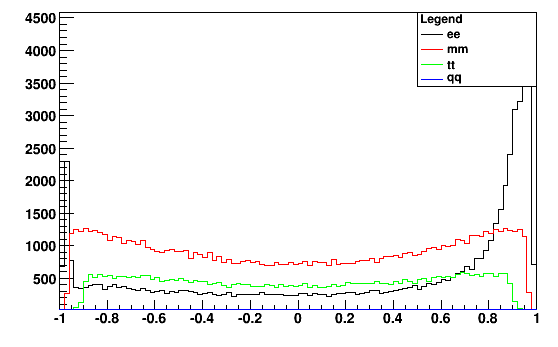
\includegraphics[width=0.49\textwidth]{../figures/cos_thet.png}}
	\caption[Verteilungen der Parameter für die Monte-Carlo-simulierten Daten]{Verteilungen der Parameter für die Monte-Carlo-simulierten Daten.}
	\label{fig:mc}
\end{figure}

\subsection{Trennung von t-Kanal und s-Kanal}

\subsection{Ermittelung der Wirkungsquerschnitte}

\subsection{Bestimmung der Partialbreiten}

\subsection{Bestimmung der Anzahl der Neutrinogenerationen}

\subsection{Bestimmung des Weinbergwinkels}